\chapter{Model checking}
\section{Introduzione}
Le \textbf{logiche temporali} sono una famiglia di logiche matematiche che
permette di esprimere proprietà che cambiano nel tempo.

Quando si analizzano sistemi reattivi (quindi concorrenti) allora non vale più
il ragionamento di avere uno stato precedente e uno stato successivo che varia
nel tempo.

Sono stati introdotti diversi modelli per modellare i sistemi concorrenti, ora
si introdurranno nuove tecniche di analisi.

Per esempio nel caso del produttore e consumatore, i soggetti sono indipendenti
quindi si devono sincronizzare per l'accesso al buffer. Per questi programmi
sarà importante garantire la correttezza del programma:
\begin{itemize}
    \item Ogni oggetto deve essere prima prodotto.
    \item Ogni oggetto non può essere consumato più di una volta.
    \item Il sistema non raggiunge mai uno stato di \textbf{deadlock}.
\end{itemize}
Le reti di Petri ci permettono di controllare se si mantiene la mutua esclusione,
ovvero che non esista una marcatura in cui entrambi i processi non possono essere
negli stati della sezione critica. Noi vorremmo modellare il blocco di uno dei
due processi se uno si trova nella zona critica.

Vogliamo quindi un modello per verificare se sono valide delle proprietà di
interesse e se il modello rappresenta effettivamente il sistema.
\begin{definizione}[\textbf{Sistema reattivo}]
    Un sistema è \textbf{reattivo} se è un sistema concorrente, distribuito e
    asincrono.
\end{definizione}
Una sottoclasse dei sistemi reattivi sono quelli sincroni con un clock, ma è una
semplificazione.

I sistemi reattivi non obbediscono più al paradigma input-computazione-output,
rendendo quindi impossibile utilizzare le triple di Hoare per dimostrare la
correttezza di un programma. Possiamo sempre riutilizzare la logica di hoare per
dimostrare alcuni pezzi, ma dovremmo usare un modo per unire i risultati.

Al posto delle triple di Hoare, utilizzeremo delle \textbf{asserzioni}, ovvero
delle frasi al cui interno sono presenti elementi temporali che descrivono il
comportamento del sistema.
\begin{esempio}
    Se è stato spedito un messaggio allora questo \textit{prima o poi} verrà
    ricevuto dal destinatario.
\end{esempio}
\begin{esempio}
    Se si accende una spia di allarme allora questa sarà accesa \textit{fino a
        quando} non si spegne il dispositivo
\end{esempio}
Vediamo ora come possiamo procedere nell'analisi dei sistemi concorrenti. Il
problema che vogliamo risolvere è quello di stabilire se un sistema reattivo è
corretto. Per fare ciò, seguiremo il seguente schema:
\begin{enumerate}
    \item Si esprime il criterio di correttezza come una formula di un opportuno
          linguaggio logico.
    \item Si modella il sistema nella forma di un sistema di transizioni.
    \item Si valuta se la formula è vera nel sistema di transizioni. (algoritmi)
\end{enumerate}
\begin{definizione}[\textbf{Sistema di transizioni}]
    Un \textbf{sistema di transizioni} è definito da:
    \begin{equation}
        A=(Q,T)
    \end{equation}
    dove:
    \begin{itemize}
        \item $Q$ insieme degli stati (non per forza finito).
        \item $T \subseteq Q \times Q$ insiemi di transizioni di stato.
    \end{itemize}
\end{definizione}
\begin{definizione}[\textbf{Cammino}]
    Definiremo un \textbf{cammino} come una sequenza di stati $\pi$ dove:
    \begin{equation}
        \pi = q_0q_1\dots q_n \ \text{dove} \ (q_i,q_{i+1})\in T \ \forall i
    \end{equation}
    (combacia con la definizione di cammino su grafi).
\end{definizione}
\begin{definizione}[\textbf{Suffisso}]
    Definiremo un \textbf{suffisso} di ordine $i$ per un cammino $\pi$ è il
    cammino che inizia da uno stato di indice $i$.
    \begin{equation}
        \pi^{(i)} = q_iq_{i+1}\dots q_n
    \end{equation}
\end{definizione}
\begin{nota}
    Posso esprimere un cammino come un suffisso di ordine 0.
\end{nota}
\begin{definizione}[\textbf{Cammino massimale}]
    Definiremo un \textbf{cammino massimale} se il cammino è finito e non può
    essere esteso, cioè solo quando il cammino raggiunge uno stato che non ha
    transizioni uscenti. (cammino massimale finito)
\end{definizione}
Il cammino massimale è infinito quando non si ha uno stato pozzo.
\begin{nota}
    Ogni suffisso di un cammino massimale è a sua volta un cammino massimale.
\end{nota}
Posso rappresentare un cammino espandendo la definizione delle espressioni
regolari, aggiungendo $^\omega$ per rappresentare una sequenza infinita. Bisogna
prestare particolare attenzione al fatto che $\omega \neq \ast$, infatti $\ast$
rappresenta una sequenza arbitraria di valori.
\section{Logica Temporale Lineare}
Definiamo la \textbf{sintassi} partendo dalle proposizioni atomiche:
\begin{equation}
    AP = \{p_1, p_2, \dots, p_i, \dots\}
\end{equation}
composte dalle asserzioni considerate vere a prescindere.
\begin{esempio}
    Il messaggio è stato spedito, la spia di allarme è accesa
\end{esempio}
\begin{definizione}[\textbf{Formule ben Formate per la logica LTL}]
    Definiamo anche le formule ben formate $FBF_{LTL}$:
    \begin{itemize}
        \item Ogni proposizione atomica è una formula ben formata.
        \item $\top$ e $\bot$ sono formule ben formate.
        \item Se $\alpha, \beta \in FBF_{LTL}$ allora $\alpha \lor \beta, \lnot
                  \alpha \in FBF_{LTL}$ (da queste si derivano tutti i connettivi
              logici).
        \item \textbf{Operatori temporali}: siano $\alpha$ e $\beta$ formule ben
              formate, allora anche:
              \begin{itemize}
                  \item $X\alpha$ "next $\alpha$" nel prossimo stato $\alpha$ è vera.
                  \item $F\alpha$ "future $\alpha$" prima o poi $\alpha$ sarà vera.
                  \item $G\alpha$ "globally $\alpha$" $\alpha$ è sempre vera.
                  \item $\alpha U \beta$ "$\alpha$ until $\beta$" $\alpha$ è vera
                        fino a quando $\beta$ diventa vera.
              \end{itemize}
              sono formule ben formate.
    \end{itemize}
\end{definizione}
Per definire la sintassi utilizzeremo i \textbf{Modelli di Kripke} che prendono
i sistemi di transizione e li arricchiscono associando a ogni stato $q \in Q$
l'insieme delle proposizioni atomiche che sono vere in $q$. Quindi possiamo
definire:
\begin{equation}
    I \ : \ Q \to 2^{AP}
\end{equation}
dove $2^{AP}$ è l'insieme delle parti di $AP$. Un modello di Kripke sarà
definito come:
\begin{equation}
    A = (Q, T, I)
\end{equation}
Con un modello di Kripke possiamo identificare per uno stato quali sono le
proposizioni atomiche vere e per capire se le $FBF_{LTL}$ sono vere allora dovrò
analizzare i cammini che partono dallo stato in esame.

Vediamo ora come associare una \textbf{semantica} alle formule ben formate. Per fare ciò
procediamo in due fasi:
\begin{enumerate}
    \item Definiamo un \textbf{criterio} per stabilire se una formula $\alpha$ è vera in
          un cammino massimale $\pi$.
    \item Diciamo che la formula è \textbf{vera} rispetto a uno stato $q$ se è vera in
          tutti i \textbf{cammini massimali} che partono da $q$.
\end{enumerate}
\begin{nota}
    Per dimostrare che una formula è vera in un determinato stato, bisogna quindi
    dimostrare che \textbf{è vera in tutti i cammini massimali} che partono da esso.
\end{nota}
Fissiamo quindi un cammino generico $\pi$ e $\alpha$ una formula ben formata allora:
\begin{equation}
    \pi \vDash \alpha \iff \ \text{significa che} \ \alpha \ \text{è vera nel cammino}
    \ \pi
\end{equation}
Definiremo la relazione $\vDash$ per induzione.
\begin{definizione} [$\vDash$]
    Supponiamo che $\alpha$ e $\beta$ siano due formule ben formate ($\alpha,
        \beta \in FbF_{LTL}$) e che  $p$ sia una preposizione atomica ($p \in AP$).
    Allora la relazione $\vDash$ è definita come:
    \begin{itemize}
        \item \textbf{caso base}:
              \begin{itemize}
                  \item $\pi \vDash \top$
                  \item $\pi \not\vDash \bot$
                  \item $\pi \vDash p \iff p\in I(q_0)$
              \end{itemize}
        \item \textbf{passo induttivo}:
              \begin{itemize}
                  \item  \textbf{Operatori logici}: supponiamo $\alpha, \beta \in FBF_{LTL}$
                        \begin{itemize}
                            \item $\pi \vDash \lnot \alpha \iff \pi \not\vDash \alpha$
                            \item $\pi \vDash \alpha \lor \beta \iff (\pi \vDash \alpha) \lor (\pi
                                      \vDash \beta) $
                        \end{itemize}
                  \item \textbf{Operatori temporali}: supponiamo $\beta, \gamma \in FBF_{LTL}$
                        \begin{itemize}
                            \item $\pi \vDash X\beta \iff \pi^{(1)}\vDash \beta$
                            \item $\pi \vDash F \beta \iff \exists i \in \mathbb{N}:
                                      \pi^{(i)} \vDash \beta$
                            \item $\pi \vDash G \beta \iff \forall i \in \mathbb{N}:
                                      \pi^{(i)} \vDash \beta$
                            \item $\pi \vDash \beta U \gamma \iff$:
                                  \begin{itemize}
                                      \item $\exists i \in \mathbb{N}$ tale che: $\pi^{(i)}
                                                \vDash \gamma$ cioè $\pi \vDash F \gamma$.
                                      \item $\forall h, 0 \leq h < i, \pi^{(h)} \vDash \beta$
                                  \end{itemize}
                                  Se $\gamma$ è vera fin da subito, quindi $i = 0$ allora
                                  $\beta$ è superfluo.
                        \end{itemize}
              \end{itemize}
    \end{itemize}
\end{definizione}
\begin{esempio}
    Ecco alcuni esempi:
    \begin{itemize}
        \item $FG\alpha$: esprime che da un certo momento in poi $\alpha$ sarà
              invariante, se $\alpha = \perp$ allo stato iniziale ma $FG\alpha =
                  \top$ vale dallo stato iniziale allora significa che non si
              tornerà più in quello stato.
        \item $GF\alpha$: $\alpha$ è vera in un numero infinito di stati.
        \item $G\lnot (cs_1\land cs_2)$: mutua esclusione se $cs_1$ indica che il
              processo è nella sezione critica, viceversa $cs_2$.
        \item $G(req \implies XF ack)$: se si manda una richiesta, dallo stato
              successivo prima o poi si riceverà un ack.
        \item $G(req \implies (req U ack))$: se c'è la richiesta allora la
              richiesta è pendente fino a quando si ha un'ack. Si differenzia da
              quella precedente dal momento che la richiesta deve rimanere fino
              a quando non si manda l'ack.
        \item $G(req \implies ((req\land \lnot ack) U (\lnot req \land ack)))$:
              si chiede di non rispondere all'inizio e dopo la risposta la richiesta
              viene cancellata.
    \end{itemize}
\end{esempio}
\begin{esempio}
    Consideriamo la seguente rete di Petri (\ref{fig:retePetriEsempio}), la
    quale rappresenta due processi che vogliono accedere ad una risorsa condivisa.
    \begin{figure}
        \centering
        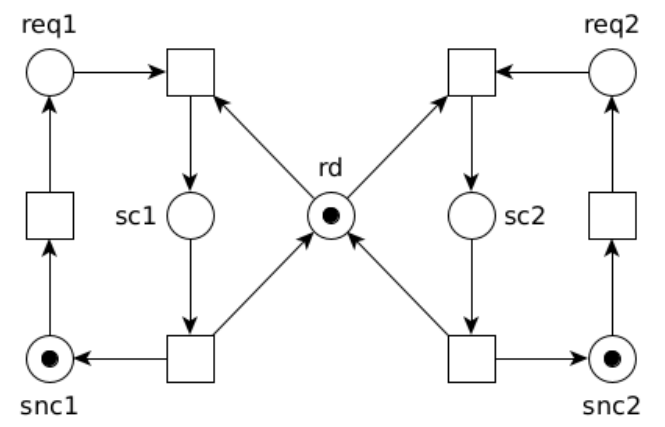
\includegraphics[width=0.5\textwidth]{img/model/retePetriEsempio.png}
        \caption{Rete di Petri per il model checking}
        \label{fig:retePetriEsempio}
    \end{figure}
    Questa rete è composta da:
    \begin{itemize}
        \item $rd$ la risorsa disponibile.
        \item $sc1$ e $sc2$ le due sezioni critiche.
        \item $snc1$ e $snc2$ le due sezioni non critiche.
        \item $req1$ e $req2$ le due richieste di usare la risorsa.
    \end{itemize}
    Per poter applicare le tecniche di model checking dobbiamo trasformare questa
    rete in un modello di Kripke. Per farlo dobbiamo definire gli stati e le
    transizioni. Una possibile soluzione è quella di calcolare il grafo dei casi
    (o grafo di raggiungibilità) della rete di Petri ed assegnare ad ogni nodo
    un insieme di proposizioni atomiche che sono vere in quel nodo.

    Possiamo quindi definire il grafo dei casi dove per semplicità utilizziamo il
    nodo $1$ come stato iniziale:
    \begin{figure}[!ht]
        \centering
        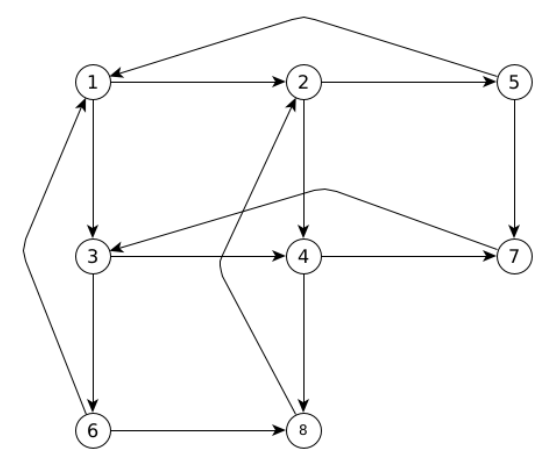
\includegraphics[width=0.5\textwidth]{img/model/GrafoDeiCasi.png}
        \caption{Grafo dei casi della rete di Petri}
    \end{figure}
    dove ogni nodo è rappresentato da:
    \begin{itemize}
        \item $1=\{rd,snc1,snc2\}$
        \item $2=\{rd,req1,snc2\}$
        \item $3=\{rd,snc1,req2\}$
        \item $4=\{rd,req1,req2\}$
        \item $5=\{sc1, snc2\}$
        \item $6=\{snc1,sc2\}$
        \item $7=\{sc1, req 2\}$
        \item $8=\{req1,sc2\}$
    \end{itemize}
    Una volta costruita la struttura, definiamo delle formule che vogliamo siano
    vere per la situazione in analisi. Studiamo quindi:
    \begin{itemize}
        \item $G \lnot (sc_1\land sc_2)$: esprime che non si può raggiungere
              uno stato in cui entrambi i processi sono nella sezione critica.
        \item $G (req1 \implies F sc1)$: esprime che se il processo 1 fa richiesta
              allora prima o poi entrerà nella sezione critica.
    \end{itemize}
    Per verificare le formule dovremmo considerare tutti i cammini massimali che
    partono dallo stato 1 e verificare che le formule siano valide in tutti i
    cammini. Tuttavia, questo caso è complesso e i possibili cammini massimali
    sono potenzialmente infiniti.

    Per la prima formula, la via più facile è, osservando che dallo stato si
    possono raggiungere tutti gli altri stati, scorrere la tabella delle formule
    vere in ciascun stato e osservare che in nessun stato è vera la formule
    $sc_1 \land sc_2$. Quindi non sarà vera globalmente.

    Per la seconda formula non possiamo più applicare questa strategia, ma
    possiamo cercare di confutare la formula: basta trovare un cammino massimale
    che non soddisfi la formula.

    In ogni caso questa seconda formula non è valida in quando potrei avere il
    cammino $\pi^{(1)}(2,4,8)^\omega$ in cui anche il secondo processo fa
    richiesta e ci entra. Posso entrare in un loop in cui solamente il processo
    due prende ogni volta la risorsa quindi la formula non è valida in quel
    cammino massimale.

    Possiamo comunque trovare cammini in cui vale, come $(1,3,6)^\omega$, in
    quanto in quei tre stati $req1$ è sempre falsa.

    Una possibile soluzione è quella di aggiungere un nuovo stato $9$, duplicando
    lo stato $4$ in modo da implementare un meccanismo di \textbf{turno} in cui
    i processi si alternano nell'uso della risorsa.
\end{esempio}
Come per tutte le logiche, anche per la logica temporale si può definire una
equivalenza tra formule.
\begin{definizione}[\textbf{Equivalenza tra formule}]
    Possiamo definire l'\textbf{equivalenza tra formule} come:
    \begin{equation}
        \alpha \equiv \beta \iff \forall \pi: ( \pi \vDash \alpha \iff
        \pi \vDash \beta)
    \end{equation}
\end{definizione}
\begin{esempio}
    Vediamo ora alcuni esempi di equivalenza tra formule:
    \begin{itemize}
        \item $F\alpha \equiv \alpha \lor XF\alpha$ se prima o poi $\alpha$ sarà
              vera, allora o è vera in questo stato oppure dal prossimo stato
              $\alpha$ sarà prima o poi vera.
        \item $G\alpha \equiv \alpha \land XG\alpha$ Se $\alpha$  è sempre vera,
              allora è vera in questo stato e dal prossimo stato sarà sempre vera.
        \item $\alpha U \beta \equiv \beta \lor (\alpha \land X(\alpha U \beta))$
              se $\beta$ è vera non ci interessa altro, oppure $\alpha$ è vera e
              dal prossimo stato $\alpha$ sarà vera fino a quando $\beta$ diventa
              vera.
        \item $FGF \alpha \equiv GF\alpha$ se prima o poi $\alpha$ sarà vera,
              allora da un certo momento in poi $\alpha$ sarà sempre vera.
        \item $GFG\alpha \equiv FG\alpha$ se $\alpha$ è sempre vera, allora da un
              certo momento in poi $\alpha$ sarà sempre vera.
        \item $\top U\alpha \equiv F\alpha$: questo significa che l'operatore
              $F$ non è essenziale.
        \item $\lnot F \lnot \alpha \equiv G \alpha$: questo significa che $G$
              può essere definito a partire da $F$ quindi l'insieme minimale di
              operazioni sono $\{X,U\}$. Questo insieme minimale non è unico.
    \end{itemize}
\end{esempio}
Le equivalenze spesso sfruttano la ricorsione dal momento che si basano su sistemi
di transizione.

Le equivalenze logiche permettono di definire degli \textbf{operatori derivati},
per velocizzare la scrittura delle formule. Alcuni esempi di operatori derivati
sono:
\begin{itemize}
    \item \textbf{Until debole}: $\alpha W \beta \equiv G\alpha \lor
              (\alpha U \beta)$ con questo operatore si può esprimere la proprietà
          in cui $\alpha$ è sempre vera oppure $\alpha$ è vera fino a quando
          $\beta$ diventa vera. $W$ differisce da $U$ perché non si richiede che
          la seconda formula diventi vera per rendere vera $W$.
    \item \textbf{Release}: $\alpha R \beta$ per cui:
          \begin{equation}
              \pi \vDash \alpha R \beta \iff \forall k \geq 0: (\pi^{(k)} \vDash
              \beta \lor \exists h < k: \pi^{(h)} \vDash \alpha)
          \end{equation}
          In sostanza o $\beta$ è sempre vera oppure $\beta$ potrà essere falsa
          solo quando $\alpha$ diventa vera. Definito in questo modo allora si
          può dire:
          \begin{equation}
              \alpha R \beta \equiv \beta W (\alpha \land \beta)
          \end{equation}
\end{itemize}
\begin{definizione}[\textbf{Insieme di operatori minimale}]
    L'insieme degli operatori è detto \textbf{minimale} se ogni altro
    operatore può essere definito a partire da questi. Un esempio di insieme di
    operatori minimale per le logiche temporali è $\{X,U\}$.
\end{definizione}
Attenzione all'uso della negazione nelle formule LTL, cosa significa "non è vero
$F\alpha$" (\textit{non è vero che prima o poi $\alpha$ diventi vera})? Significa
che $\exists$ un cammino per cui non vale $F\alpha$. Mentre $\lnot F\alpha \equiv
    G\lnot \alpha$ quindi $\lnot F\alpha$ non è la negazione di $F\alpha$. Quindi
dobbiamo stare attenti ai quantificatori universali nascosti.

Negli esercizi sulla logica temporale ci possono essere diverse risposte giuste.
Ecco degli esercizi sulla logica temporale lineare.
\begin{esempio}
    Traduci questa frase:
    \begin{center}
        Chi ruba, presto o tardi finirà in galera.
    \end{center}
    possiamo considerare 2 proposizioni atomiche:
    \begin{itemize}
        \item $hr$: ho rubato
        \item $c$: sono in carcere
    \end{itemize}
    Si può riformulare la frase come una legge, quindi come una cosa che vale
    sempre, portandoci ad utilizzare l'operatore $G$. In aggiunta, possiamo
    riformularla in un modo che ha una semantica più vicina alla semantica degli
    operatori logici.
    \begin{center}
        Se rubi, in futuro finirai in galera.
    \end{center}
    Si può tradurre in
    \begin{equation}
        G(hr \implies XF \ c)
    \end{equation}
    Utilizziamo l'operatore $X$ per evitare che nel momento in cui rubo allora
    subito finisco in galera.

    Possiamo provare a tradurre la frase
    \begin{center}
        Solo chi ruba finirà in galera.
    \end{center}
    Quindi si può tradurre
    \begin{equation}
        \lnot c \ W \ hr \equiv G(c \iff hr)
    \end{equation}
\end{esempio}
\begin{esempio}
    Traduci questa frase:
    \begin{center}
        Chi ruba finirà in carcere, ma solo dopo avere parlato con un avvocato.
    \end{center}
    si aggiunge anche la proposizione atomica: "ho parlato con un avvocato"
    \begin{equation}
        G(hr\implies (XF \ c \land (\lnot c \ U \ pa)))
    \end{equation}
    Si potrebbe pensare che $XF \ c$ si possa escludere ma in realtà no perché
    $U$ porta a dire che dopo aver parlato con un avvocato non vuol dire che $c$
    diventi vera.
\end{esempio}
\begin{esempio}
    Traduci questa frase:
    \begin{center}
        Se la cabina è in movimento verso l'alto, si trova all'altezza del
        secondo piano, ed è stato premuto il pulsante interno di richiesta del
        quinto piano, allora la cabina non cambierà direzione fino a quando avrà
        raggiunto il quinto piano.
    \end{center}
    si specificano le proposizioni atomiche:
    \begin{itemize}
        \item $su$: "la cabina sta salendo"
        \item $p_i$: "cabina all'altezza del piano $i$"
        \item $r_i$: "pulsante interno del piano $i$ è stato premuto"
    \end{itemize}
    \begin{equation}
        G((su \land p_2 \land r_5)\implies(su \ U \ p_5))
    \end{equation}
\end{esempio}
La logica temporale che abbiamo studiato fino a questo momento (LTL) permette di
esprimere diverse proprietà dei sistemi reattivi, ma ha dei limiti, infatti non
permette di esprimere proprietà del tipo:
\begin{center}
    \emph{``esiste un cammino in cui vale $\alpha$''}
\end{center}
Attraverso le formule della logica LTL possiamo esprimere solo proprietà in cui
si richiede che una certa formula sia vera \textit{in tutti} i cammini massimali.
Non possono essere espresse proprietà relative all'esistenza di un cammino in cui
una certa formula è vera.

Il problema è che queste proprietà sono utili, per risolvere questa mancanza
introduciamo una nuova logica. Questa logica può essere interpretata attraverso
il concetto di \textbf{albero di computazione}.
\begin{definizione}[\textbf{Albero di computazione}]
    Un \textbf{albero di computazione} è una struttura che mi permette di
    rappresentare le possibili computazioni di un sistema di transizioni
    etichettato.

    I cammini che partono dalla radice di questo albero sono definiti come
    \textbf{computazioni} del sistema. Un esempio di albero di computazione è
    riportato in figura \ref{fig:computational-tree-logic}
\end{definizione}
\begin{nota}
    Spesso si vuole esprime le possibili computazioni di un sistema allora
    possiamo costruire un albero (simile all'\textbf{unfolding} per le reti di
    petri) che rappresenta la computazione rispetto gli stati globali.

    L'albero può essere costruito in modo induttivo:
    \begin{itemize}
        \item Si sceglie lo stato iniziale.
        \item Se si hanno transizioni verso altri stati allora li aggiungo come
              prossimi nodi.
        \item Così via ricorsivamente, se ci sono archi all'indietro allora
              si ricrea un altro nodo in avanti.
    \end{itemize}
    Nel caso fosse ciclico allora sarà infinito, se abbiamo stati in deadlock
    allora il nodo sarà pozzo.
\end{nota}
\begin{figure}[!ht]
    \centering
    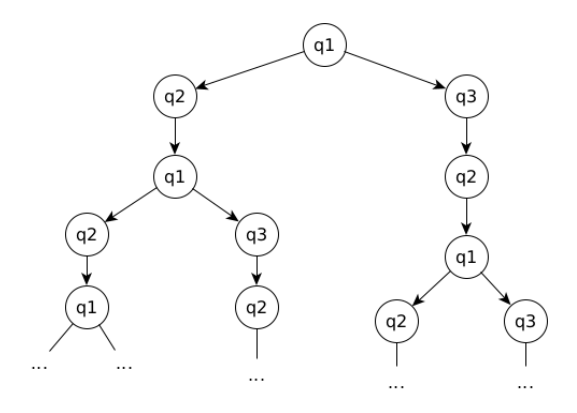
\includegraphics[width=0.5\textwidth]{img/model/computational-tree-logic.png}
    \caption{Esempio di computational tree}
    \label{fig:computational-tree-logic}
\end{figure}
\section{Computation Tree Logic - CTL}
Possiamo definire ora la logica CTL (\textbf{Computation Tree Logic}), ovvero
una logica temporale che si basa sugli alberi di computazione.

Definiremo la \textbf{sintassi} attraverso le $FbF_{CTL}$.
\begin{definizione}[\textbf{Formule ben Formate per la logica CTL}]
    Le formule ben formate sono:
    \begin{itemize}
        \item $\forall p \in AP, p\in FbF_{CTL}$ con $AP = \{p_1,p_2,\dots\}$
              insieme delle preposizioni atomiche.
        \item $\forall \alpha, \beta \in FbF_{CTL}$
              \begin{itemize}
                  \item $\lnot\alpha, \alpha \lor \beta \in FbF_{CTL}$
                  \item $AX \ \alpha, EX \ \alpha \in FbF_{CTL}$ per ogni / esiste
                        un cammino dallo stato corrente tale che nello stato prossimo
                        vale $\alpha$
                  \item $AF \ \alpha, EF \ \alpha \in FbF_{CTL}$ per ogni / esiste
                        un cammino dallo stato corrente tale che prima o poi vale $\alpha$
                  \item $AG \ \alpha, EG \ \alpha \in FbF_{CTL}$ per ogni / esiste
                        un cammino dallo stato corrente tale che vale sempre $\alpha$
                  \item $A(\alpha \ U \ \beta), E(\alpha \ U \ \beta)\in FbF_{CTL}$
                        per ogni / esiste un cammino dallo stato corrente tale che
                        $\alpha$ è vera fino a quando $\beta$ non diventa vera.
                        ($\beta$ deve per forza diventare vera)
              \end{itemize}
    \end{itemize}

\end{definizione}
In particolare, abbiamo aggiunto $A$ e $E$ i quali rappresentano due quantificatori
sui cammini. Essi sono definiti come segue:
\begin{itemize}
    \item $A\equiv \forall$ è il quantificatore universale e si interpreta come
          \textbf{per ogni cammino}.
    \item $E\equiv \exists$ è il quantificatore esistenziale e si interpreta come
          \textbf{esiste un cammino tale che}.
\end{itemize}
\begin{osservazione}
    Nelle formule della logica CTL, i quantificatori $A$ ed $E$ devono essere
    sempre presenti quando si ha un operatore temporale.
\end{osservazione}
\begin{esempio}
    Traduciamo
    \begin{center}
        Dopo l'accensione della spia, sarà sempre possibile riportare il sistema
        allo stato iniziale.
    \end{center}
    Definiamo:
    \begin{itemize}
        \item $s$: la spia è accesa
        \item $init$: il sistema si trova nello stato iniziale
    \end{itemize}
    \begin{equation}
        AG(s\implies AX \ EF \ init)
    \end{equation}
\end{esempio}
\begin{esempio} [Esercizio d'esame]
    Dato il sistema di transizione riportato in figura \ref{fig:esercizioEsame},
    vogliamo verificare la seguente proprietà:
    \begin{itemize}
        \item $AF \ q$
        \item $AG (EF (p \lor q))$, $GF(p \lor q)$
        \item $EX (EX \ r)$, $XX \ r$
        \item $AG (AF \ q)$
    \end{itemize}
    \begin{figure}[!ht]
        \centering
        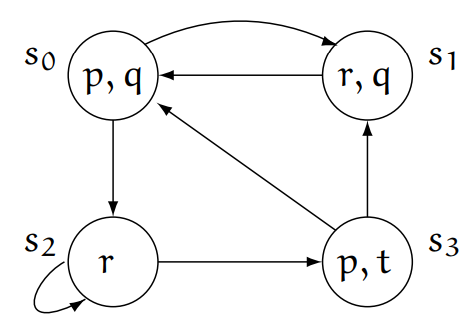
\includegraphics[width=0.5\textwidth]{img/model/esercizioEsame.png}
        \caption{Sistema di transizione}
        \label{fig:esercizioEsame}
    \end{figure}
    Vediamo ora come risolvere i vari punti:
    \begin{itemize}
        \item $AF \ q$: in questo caso conviene suddividere la formula ed
              analizzare gli elementi semplici, come $F$ e $q$. A questo punto
              controlliamo per ogni stato dove vale $q$, in questi stati, per
              come abbiamo definito $F$ la formula risulta vera. Quindi negli
              stati $s_0$ e $s_1$ la formula è vera. Successivamente verifico se
              sui cammini che partono dagli altri stati $q$ diventa vera. Questo
              è vero per il cammino che parte da $S_3$, ma non per quello che parte
              da $s_2$, dal momento che in quest'ultimo stato è presente un
              cappio quindi può non andare mai in $s_3$.
        \item $GF(p \lor q)$: avendo questa formula non basta analizzare dove
              valgono $p$ o $q$ perché abbiamo $G$ quindi dobbiamo controllare
              anche che per tutti gli stati successivi $p$ o $q$ siano vere.
              Detto ciò, possiamo osservare che la formula è falsa in tutti gli
              stati in quanto per ognuno è possibile definire un cammino che
              arriva nello stato $s_2$ dove la formula $p \lor q$ è falsa.
        \item $AG (EF (p \lor q))$: è vera per tutti gli stati perché esiste
              sempre un cammino con una deviazione in cui vale $p \lor q$.
        \item $XX \ r$: non è vera in $s_0$ perché abbiamo trovato un cammino
              per cui non è vera $s_0\to s_1\to s_0$. Mentre $s_1$ è verificata.
        \item $EX (EX \ r)$: è vera in $s_0$ perché abbiamo trovato un cammino
              per cui è vera $s_0\to s_2\to s_2$ e a noi ne basta una sola.
        \item $AG (AF \ q)$: non vale in $s_2$ perché possiamo rimanere
              all'infinito, Mentre negli altri è sempre vera.
    \end{itemize}
\end{esempio}
\begin{nota}
    Ricorda che per la semantica della logica $LTL$ allora alcune delle $FbF_{LTL}$
    sono equivalenti alle $FbF_{CTL}$ che hanno l'operatore $A$ e viceversa.

    Per esempio
    \begin{equation}
        AF\alpha \equiv F\alpha
    \end{equation}
\end{nota}
Anche per questa logica definiremo l'equivalenza logica.
\begin{definizione}[\textbf{Formule equivalenti}]
    Due formule $\alpha$ e $\beta$ sono equivalenti, indicato come $\alpha \equiv
        \beta$, se e solo se:
    \begin{equation}
        \forall \pi \land \forall \models : (\pi \models \alpha \iff \pi \models
        \beta)
    \end{equation}
\end{definizione}
In entrambe le logiche, LTL e CTL, possiamo esprimere le seguenti proprietà:
\begin{itemize}
    \item \textbf{Invariante}: si possono avere delle formule sempre vere:
          \begin{equation}
              AG\lnot p \equiv G\lnot p
          \end{equation}
    \item \textbf{Reattiva}: il valore logico di una formula implica la veridicità
          di un'altra:
          \begin{equation}
              AG (p\implies AF \ q) \equiv G(p\implies F \ q)
          \end{equation}
\end{itemize}
Le due logiche non hanno la stessa potenza espressiva ma nessuna delle due è più
espressiva rispetto all'altra. Infatti per esempio la logica CTL può esprimere
la seguente proprietà (\textbf{reset property}):
\begin{center}
    Da ogni stato raggiungibile in ogni cammino è sempre possibile raggiungere
    uno stato nel quale vale $p$.
\end{center}
Esprimibile secondo la seguente formula $AG \ EF \ p$, per cui non esiste una formula
LTL che possa esprimere la proprietà.

Al contrario la logica LTL può esprimere la seguente proprietà:
\begin{center}
    In ogni cammino, prima o poi si raggiungerà uno stato a partire dal quale $p$
    rimane sempre vera.
\end{center}
Esprimibile secondo la seguente formula $F \ G \ p$, per cui non esiste una formula
CTL che possa esprimere la proprietà.

Quindi CTL e LTL sono delle logiche temporali che hanno poteri espressivi diversi,
ovvero esistono formule che possono essere espresse in una logica ma non nell'altra.

Per ovviare a questo problema si definisce l'estensione di CTL (CTL$^\ast$),
in particolare, si rimuove dalla logica CTL il vincolo di avere un quantificatore
che precede ogni operatore temporale.

Lo svantaggio di questa logica è che richiede un maggiore sforzo computazionale
per dimostrare le proprietà, sarà quindi importante decidere quale logica usare.
\begin{figure}[!ht]
    \centering
    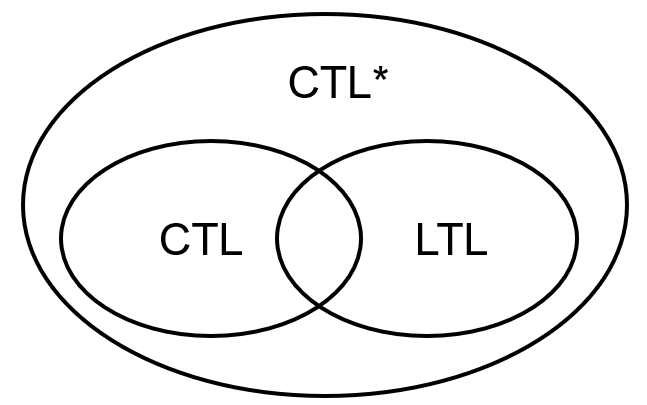
\includegraphics[width=0.3\textwidth]{img/model/logicheTemprali.png}
    \caption{Relazione tra le logiche temporali}
\end{figure}

Come abbiamo dimostrato quando sono equivalenti le FbF, potremmo anche voler
controllare se due modelli di Kripke sono equivalenti. Ragionevolmente si potrebbe
pensare all'equivalenza dei modelli di Kripke solo quando sono isomorfi, ciò
è troppo restrittivo.
\begin{definizione}[\textbf{Equivalenza tra modelli}]
    Diremo due modelli $M_1$ e $M_2$, con stati iniziali $q_0$ e $s_0$, si dicono
    \textbf{equivalenti} rispetto a una logica $L$ se, $\forall \alpha \in FbF_L$
    vale che:
    \begin{equation}
        M_1, q_0 \models \alpha \iff M_2, s_0 \models \alpha
    \end{equation}
\end{definizione}
Per dimostrare che due modelli sono equivalenti devo:
\begin{itemize}
    \item Definire tutti i cammini massimali di $M_1$ e $M_2$ nella forma simile
          alle regex e si rimuovono i duplicati.
    \item Trasformare le espressioni ottenute sostituendo i nomi degli stati con
          le preposizioni atomiche che sono vere in un determinato stato.
    \item Se le espressioni dei cammini massimali di un modello sono uguali
          all'altro allora i due modelli sono equivalenti.
\end{itemize}
\begin{esempio}
    Vediamo ora un esempio per dimostrare che due modelli sono equivalenti.
    Consideriamo i modelli $M_1$ e $M_2$ riportati in figura \ref{fig:esempioModelli}.
    \begin{figure}[!ht]
        \centering
        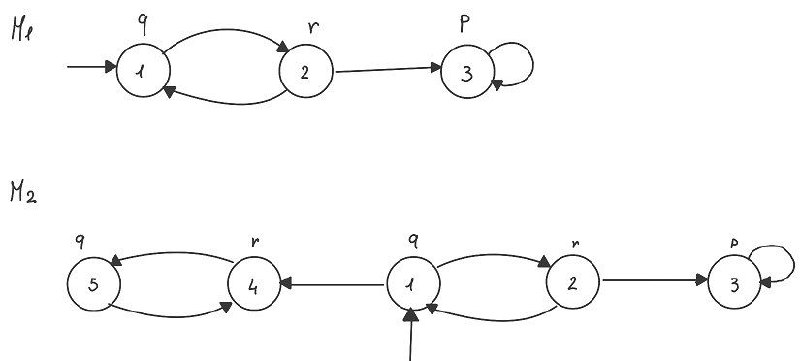
\includegraphics[width=0.5\textwidth]{img/model/esempioEquivalenzaModelli.png}
        \caption{Modelli da confrontare}
        \label{fig:esempioModelli}
    \end{figure}
    Per verificare l'equivalenza dobbiamo:
    \begin{itemize}
        \item Costruire i cammini massimali dei due modelli.
              \begin{itemize}
                  \item Modello $M_1$:
                        \begin{equation}
                            \begin{array}{l}
                                (1 \ 2)^\omega \\
                                (1 \ 2)^\ast \ 3^\omega
                            \end{array}
                        \end{equation}
                  \item Modello $M_2$:
                        \begin{equation}
                            \begin{array}{l}
                                1 \ (4 \ 5)^\omega      \\
                                (1 \ 2)^{\omega}        \\
                                (1 \ 2)^\ast \ 3^\omega \\
                                (1 \ 2)^\ast \ 1 \ (4 \ 5)^\omega
                            \end{array}
                        \end{equation}
              \end{itemize}
        \item Sostituire i nomi degli stati con le preposizioni atomiche che sono
              vere in un determinato stato.
              \begin{itemize}
                  \item Modello $M_1$:
                        \begin{equation}
                            \begin{array}{l}
                                (\{q\} \ \{r\})^\omega \\
                                (\{q\} \ \{r\})^\ast \ \{p\}^\omega
                            \end{array}
                        \end{equation}
                  \item Modello $M_2$:
                        \begin{equation}
                            \begin{array}{l}
                                \{q\} \ (\{r\} \ \{q\})^\omega = (\{q\} \
                                \{r\})^\omega                       \\
                                (\{q\} \ \{r\})^{\omega}            \\
                                (\{q\} \ \{r\})^\ast \ \{p\}^\omega \\
                                (\{q\} \ \{r\})^\ast \ \{q\} \ (\{r\} \
                                \{q\})^\omega = (\{q\} \ \{r\})^\omega
                            \end{array}
                        \end{equation}
              \end{itemize}
        \item Verificare che le espressioni dei cammini massimali dei due modelli.
    \end{itemize}
\end{esempio}
\begin{nota}
    Il numero dei casi raggiungibili di una rete di petri è $\leq |P(c_{in})|$,
    se gli eventi abilitati sono indipendenti allora $|C_\Sigma| = |P(c_{in})|$.
\end{nota}
\section{Insiemi parzialmente ordinati}
\begin{definizione}[\textbf{Relazione d'ordine parziale}]
    Definiremo una \textbf{relazione d'ordine parziale} su un insieme $A$ una
    relazione binaria definita come:
    \begin{equation}
        \leq \subseteq A \times A
    \end{equation}
    Allora $\leq$ deve soddisfare le seguenti proprietà:
    \begin{itemize}
        \item \textbf{Riflessiva}: $\forall x \in A, x \leq x$
        \item \textbf{Antisimmetrica}: $\forall x, y \in A, x \leq y \land y
                  \leq x \implies x = y$
        \item \textbf{Transitiva}: $\forall x, y, z \in A, x \leq y \land y \leq
                  z \implies x \leq z$
    \end{itemize}
\end{definizione}
Inoltre $x \geq y \equiv y \leq x$, possiamo definire un ordine completo ovvero
$x < y$ che vuol dire che $x \leq y \land x \neq y$.
\begin{osservazione}
    La più piccola relazione d'ordine parziale è la relazione identità.
\end{osservazione}
%% TODO: Altre osservazioni
Raffinamento di una relazione d'ordine parziale:
\begin{definizione}[\textbf{Maggiorante, Minorante}]
    Sia $(A,\leq)$ un insieme parzialmente ordinato e $B \subseteq A$ allora:
    \begin{itemize}
        \item $x \in A$ è un \textbf{maggiorante} di $B$ se $\forall y \in B, y
                  \leq x$
        \item $x \in A$ è un \textbf{minorante} di $B$ se $\forall y \in B, x
                  \leq y$
    \end{itemize}
    Può essere che $x \in B$ perché $B \subseteq A, x \in B \implies x \in A$.
\end{definizione}
Utilizziamo la notazione $B^\ast$ per indicare l'insieme dei maggioranti di $B$,
e $B_\ast$ per indicare l'insieme dei minoranti di $B$. Inoltre, diremo che:
\begin{itemize}
    \item $B$ è \textbf{limitato superiormente} se $B^\ast \neq \emptyset$
    \item $B$ è \textbf{limitato inferiormente} se $B_\ast \neq \emptyset$
\end{itemize}
\begin{definizione}[\textbf{Massimo, Minimo, Massimale, Minimale}]
    Sia $(A,\leq)$ un insieme parzialmente ordinato e $B \subseteq A$:
    \begin{itemize}
        \item Se $x \in B$ è il \textbf{minimo} di $B$ se $x \leq y, \forall y
                  \in B$, quindi $x$ è anche un \textbf{minorante} per $B$. (max 1)
        \item Se $x \in B$ è il \textbf{massimo} di $B$ se $x \geq y,\forall y
                  \in B$, quindi $x$ è anche un \textbf{maggiorante} per $B$. (max 1)
        \item Se $x \in B$ è il \textbf{minimale} in $B$ se $x \geq y \implies
                  x = y$.
        \item Se $x \in B$ è il \textbf{massimale} in $B$ se $x \leq y \implies
                  x = y$.
    \end{itemize}
\end{definizione}
\begin{definizione}[\textbf{Estremo superiore, Estremo inferiore}]
    Se $x$ è il minimo di $B^\ast$ (quindi il più piccolo maggiorante), diciamo
    che $x$ è l'\textbf{estremo superiore} (\textit{join}) di $B$, e scriviamo
    $x = \sup B$ , o anche $x = \bigvee B$.

    Se $x$ è il massimo di $B_\ast$ (quindi il più grande minorante), diciamo che
    $x$ è l'\textbf{estremo inferiore} (\textit{meet}) di $B$, e scriviamo $x =
        \inf B$ , o anche $x = \bigwedge B$.

    In particolare, se $B = \{x, y\}$, scriveremo $x \lor y$ per indicare $\bigvee
        B$, se esiste, e $x \land y$ per $\bigwedge B$.
\end{definizione}
\begin{esempio}
    Consideriamo i seguenti esempi:
    \begin{itemize}
        \item $(2^A, \subseteq)$: potremo dire che l'estremo superiore è l'unione
              mentre l'estremo inferiore è l'intersezione.
        \item $(\mathbb{N}^+,|)$: potremmo dire che l'estremo inferiore è MCD, Mentre
              l'estremo superiore è mcm.
    \end{itemize}
\end{esempio}
Le relazioni di ordine parziale possiamo rappresentarle come diagrammi di Hasse,
in cui si rappresentano le relazioni mostrando i collegamenti col successivo,
senza rappresentare la riflessività e la transitività.
\begin{definizione}[\textbf{Reticolo}]
    Definiremo un \textbf{reticolo} come un insieme parzialmente ordinato $(L,
        \leq)$, tale che, per ogni $x,y\in L$ esistono l'estremo superiore ($x
        \lor y$) e l'estremo inferiore ($x \land y$).
\end{definizione}
Per i reticoli si può dimostrare per induzione che per ogni coppia esiste il join
e il meet.
\begin{definizione}[\textbf{Reticlo completo}]
    Un reticolo si dice \textbf{completo} se per ogni sottoinsieme finito esistono
    il meet e join.
\end{definizione}
\begin{definizione}[\textbf{Funzione monotona}]
    Siano due insiemi parzialmente ordinati $(A,\leq)$ e $(B,\leq)$. Definiremo
    una funzione di $f: A \to B$ si dice \textbf{monotona} se, per ogni $x, y
        \in A$, allora:
    \begin{equation}
        x \leq y \implies f(x) \leq f(y)
    \end{equation}
    In altri termini, dati due insiemi parzialmente ordinati allora una funzione
    è monotona se mantiene l'ordine dal dominio al codominio.
\end{definizione}
\begin{definizione}[\textbf{Punto fisso}]
    Data una funzione $f: X \to X$, un elemento $x \in X$ si dice \textbf{punto
        fisso} di $f$ se $f(x) = x$.
\end{definizione}
\begin{esempio}
    Vediamo alcuni esempi di punti fissi:
    \begin{itemize}
        \item $f: \mathbb{R} \to \mathbb{R}$ $f(x) = x^2$ ha due punti fissi,
              $0$ e $1$.
        \item $g: \mathbb{R} \to \mathbb{R}$ $g(x) = \log(x)$ non ha punti fissi
              ($\emptyset$).
        \item $h: \mathbb{R} \to \mathbb{R}$ $h(x) = x$ l'insieme dei punti fissi
              è: $\mathbb{R}$.
    \end{itemize}
\end{esempio}
A noi interesseranno le funzioni monotone da un insieme su se stesso.
Se $(A, \leq)$ è un insieme parzialmente ordinato, e $f: A \to A$ è una funzione
monotona, possiamo chiederci se esistano un minimo e un massimo punto fisso.
\begin{esempio}
    Consideriamo $A = 2^\mathbb{N}$ e $S\subseteq \mathbb{N}$, $f(S)=S\cup \{2,7\}$.
    Tutti i punti fissi sono gli insiemi che contengono $\{2,7\}$, il minimo è
    $\{2,7\}$, il massimo è $\mathbb{N}$.
\end{esempio}
\begin{teorema}[\textbf{Knaster-Tarski}]
    Sia $(L,\leq)$ un reticolo completo e $f: L \to L$ sia una funzione monotona.
    Allora $f$ ha un minimo e un massimo punto fisso.
    \begin{proof}
        Analizziamo la dimostrazione nel caso particolare in cui $L = \mathcal{P}(A)$
        e $f: \mathcal{P}(A) \to \mathcal{P}(A)$ è monotona.

        L'esistenza del minimo punto fisso viene dimostrata nei seguenti passaggi:
        \begin{enumerate}
            \item Costruiamo l'insieme $Z = \{T \subseteq A \mid f(T) \subseteq
                      T\}$. Gli elementi di questo insieme $Z$ saranno chiamati
                  \textbf{punti pre-fissi}. È importante notare che l'insieme $Z$
                  non può essere vuoto, in quanto $A \in Z$. Inoltre, se $f$ ha
                  dei punti fissi $Z$ li contiene tutti.
            \item A questo punto poniamo $m = \bigcap Z$ dal momento che $Z \neq
                      \emptyset$
            \item Per ogni $S \in Z$ allora $m \subseteq S$, per di più sapendo
                  che $f$ è monotona possiamo dire che:
                  \begin{equation}
                      f(m) \subseteq f(S)
                  \end{equation}
            \item Inoltre, per definizione di $f$ abbiamo che $f(S) \subseteq S$
                  allora per la transitività di $\subseteq$ abbiamo:
                  \begin{equation}
                      f(m) \subseteq f(S) \subseteq S
                  \end{equation}
            \item Dal punto precedente possiamo arrivare a dire che $f(m) \subseteq
                      \bigcap Z = m$, questo perché se $f(m)$ è un sottoinsieme di
                  tutti i sottoinsiemi di $Z$ sarà un sotto insieme della loro
                  intersezione, quindi $m \in Z$ ed è il minimo.
            \item Vogliamo ora dimostrare che sia punto fisso. Sapendo che
                  $f(m) \subseteq m$ possiamo dire che:
                  \begin{equation}
                      f(f(m)) \subseteq f(m)
                  \end{equation}
                  quindi per definizione di $Z$ sappiamo che $f(m)\in Z$.
            \item Dal momento che $m$ è il più piccolo elemento di $Z$ abbiamo:
                  \begin{equation}
                      m \subseteq f(m) \implies m = f(m)
                  \end{equation}
                  quindi è un punto fisso, inoltre, è il punto fisso minimo.
        \end{enumerate}
        Possiamo fare il ragionamento speculare per dimostrare il massimo punto
        fisso, in questo caso al posto che usare $\bigcap$ con $\bigcup$ e $\subseteq$
        e poi avremo \textbf{post-fissi}.

        L'esistenza del massimo punto fisso viene dimostrata nei seguenti passaggi:
        \begin{enumerate}
            \item Costruiamo l'insieme $Z = \{T\in Z \mid  T \subseteq A \land T \subseteq
                      f(T) \}$. Gli elementi di questo insieme $Z$ saranno chiamati
                  \textbf{punti post-fissi}. È importante notare che l'insieme $Z$
                  non può essere vuoto, in quanto $A \in Z$. Inoltre, se $f$ ha
                  dei punti fissi $Z$ li contiene tutti.
            \item A questo punto poniamo $M = \bigcup Z$ dal momento che $Z \neq
                      \emptyset$
            \item Per ogni $S \in Z$ allora $S\subseteq M$, per di più sapendo
                  che $f$ è monotona possiamo dire che:
                  \begin{equation}
                      f(S) \subseteq f(M)
                  \end{equation}
            \item Inoltre, per definizione di $f$ abbiamo che $S \subseteq f(S)$
                  allora per la transitività di $\subseteq$ abbiamo:
                  \begin{equation}
                      S \subseteq f(S) \subseteq M
                  \end{equation}
            \item Dal punto precedente possiamo arrivare a dire che $M = \bigcup Z \subseteq
                      f(M)$, questo perché l'unione appartiene a $Z$ per definizione,
                  quindi $M \in Z$ ed è il massimo.
            \item Vogliamo ora dimostrare che sia punto fisso. Sapendo che
                  $M \subseteq f(M)$ possiamo dire che:
                  \begin{equation}
                      f(M) \subseteq f(f(M))
                  \end{equation}
                  quindi per definizione di $Z$ sappiamo che $f(M)\in Z$.
            \item Dal momento che $M$ è il più grande elemento di $Z$ abbiamo:
                  \begin{equation}
                      f(M) \subseteq M \implies M = f(M)
                  \end{equation}
                  quindi è un punto fisso, inoltre, è il punto fisso massimo.
        \end{enumerate}
    \end{proof}
\end{teorema}
Sfruttando il teorema di Knaster-Tarski possiamo ottenere il seguente teorema:
\begin{teorema}[\textbf{Teorema di Kleene}]
    Sia $f:2^A \to 2^A$ monotona allora diremo che $f$ è \textbf{continua} se
    \begin{equation}
        X_1 \subseteq X_2 \subseteq \dots \subseteq X_n \subseteq \dots
    \end{equation}
    e come conseguenza del fatto che sia monotona si ha anche:
    \begin{equation}
        f(X_1) \subseteq f(X_2) \subseteq \dots \subseteq f(X_n) \subseteq \dots
    \end{equation}
    allora:
    \begin{equation}
        f(\bigcup_{i=1}^{\infty} X_i) = \bigcup_{i=1}^{\infty} f(X_i)
    \end{equation}
\end{teorema}
Ci interessa la continuità della funzione perché, se $f$ è continua, allora:
\begin{itemize}
    \item Il minimo punto fisso di $f$ si può ottenere calcolando ricorsivamente
          $f(\emptyset)$ fino a quando non troviamo il primo punto fisso.
          \begin{equation}
              f(\emptyset), f(f(\emptyset)), f(f(f(\emptyset))), \dots
          \end{equation}
    \item Il massimo punto fisso di $f$ si può ottenere calcolando ricorsivamente
          $f(A)$ fino a quando non troviamo il primo punto fisso.
          \begin{equation}
              f(A), f(f(A)), f(f(f(A))), \dots
          \end{equation}
\end{itemize}
Possiamo legare questi teoremi alle logiche temporali CTL per avere un algoritmo
di dimostrazione della formula. Supponiamo $AFp$, partiamo dall'insieme in cui
tutti gli stati è vera $p$, allarghiamo questo insieme agli elementi che portano in
questo insieme allora $AFp$ vale sempre. Ripeto questa operazione fino a quando
non posso aggiungere altri stati (punto fisso). Il problema è trovare questa
funzione $f$ che mi permetta di applicare questo algoritmo. Per una formula $Gp$
è il contrario, si parte dall'insieme di stati per cui non vale $p$ e ricorro da
quali stati ricado in questa regione fino a quando non cambia nulla, il risultato
è l'insieme complemento.
\subsection{Algoritmo per CTL}
Sia $M=(Q,T,I)$ un modello di Kripke, allora posso definire:
\begin{definizione}[\textbf{Estensione}]
    Sia $\alpha$ una formula CTL, definiamo l'\textbf{estensione} di $\alpha$ come:
    \begin{equation}
        [[\alpha]] = \{q \in Q \mid M, q \models \alpha\}
    \end{equation}
    ovvero l'insieme degli stati in cui vale la formula $\alpha$.
\end{definizione}
A questo punto consideriamo la formula $\alpha \equiv A F \beta$, a cui è associata
la funzione $f_\alpha: \mathcal{P}(Q) \to \mathcal{P}(Q)$. Per ogni $H \subseteq Q$
si ha:
\begin{equation}
    f_\alpha(H) = [[\beta]] \cup \{q \in Q \mid \forall(q, q') \in T: q ' \in H\}
\end{equation}
\begin{osservazione}
    $f_\alpha (\emptyset) = [[\beta]]$.
\end{osservazione}
Definita in questo modo allora $f$ è monotona e continua, quindi possiamo usare
l'algoritmo per ottenere il minimo punto fisso di insiemi per cui vale la formula.
\begin{center}
    $[[\alpha]]$ è il minimo punto fisso di $f_\alpha$.
\end{center}

Col medesimo ragionamento possiamo considerare la formula  $\alpha \equiv E G
    \beta$, a cui è associata la funzione $g_\alpha: \mathcal{P}(Q) \to \mathcal{P}(Q)$.
Per ogni $H \subseteq Q$ si ha:
\begin{equation}
    g_\alpha(H) = [[\beta]] \cap \{q \in Q \mid \exists(q, q') \in T: q ' \in H\}
\end{equation}
\begin{osservazione}
    $g_\beta (Q) = [[\beta]]$.
\end{osservazione}
In questo caso cercheremo il massimo punto fisso di stati per cui non vale la
formula.
\begin{center}
    $[[\alpha]]$ è il massimo punto fisso di $g_\alpha$.
\end{center}
Dal momento che abbiamo visto l'insieme degli operatori minimali allora,
ragionando secondo un algoritmo, allora definiremo solo una funzione per $X$ e
una per $U$ per la dimostrazione e poi trasformeremo le formule in quegli operatori.
\begin{nota}
    Cerca la funzione che dimostra $A(\alpha U \beta)$ portalo all'orale.
\end{nota}
Definiamo una funzione per $\gamma \equiv A(\alpha U \beta)$, cioè $f_\gamma$:
\begin{equation}
    f_\gamma(H) = [[\beta]] \cup \{q\in [[\alpha]] \mid \forall (q, q')\in T, q'\in H\}
\end{equation}

\begin{nota}
    Ricorda che $H$ contiene tutti gli stati dove è vera la formula che si sta cercando
    di dimostrare.
\end{nota}
\section{Algoritmi per il model checking}
Precedentemente è stato introdotto un algoritmo per verificare se una formula della
logica $CTL$ è valida, ciò è possibile mediante un modello di Kripke e una funzione
monotona, utilizzando i punti fissi.

Questo ragionamento non si può riutilizzare per la dimostrazione di formule della
logica $LTL$, dal momento che non vale più il ragionamento dei punti fissi.
\begin{nota}
    Non possiamo applicare l'algoritmo per le formule della logica $CTL$ per la
    dimostrazione delle formule della logica $LTL$.
\end{nota}
Vogliamo quindi trovare un algoritmo che dato un modello di Kripke, definito sulle
proposizioni atomiche $AP$, e una formula della logica $LTL$ ci dice se tale
formula è verificata nello stato iniziale.

Tale algoritmo si basa su un automa a stati finiti che riconosce parole infinite
su un alfabeto finito $\Sigma$, tale automa è anche noto come \textbf{automa di
    Büchi}.
\begin{definizione}[\textbf{Automa di Büchi}]
    Definiamo l'\textbf{automa di Büchi} come una quadrupla:
    \begin{equation}
        \mathcal{B} = (Q, q_0, \delta, F)
    \end{equation}
    dove:
    \begin{itemize}
        \item $Q$ è un insieme finito di stati, anche dette locations.
        \item $q_0 \in Q$ è lo stato iniziale.
        \item $\delta \subseteq Q \times \Sigma \times Q$ è una relazione di
              transizione.
        \item $F \subseteq Q$ è l'insieme degli stati accettanti.
    \end{itemize}
\end{definizione}
Si trasforma il problema in un'accettazione di linguaggi di parole infinite,
riconoscibili mediante gli automi sopracitati. Però in questi linguaggi cambia il
metodo di accettazione delle parole, dal momento che l'esecuzione dell'automa non
può finire in uno stato accettante.
\begin{definizione}[\textbf{Accettazione di una parola infinita}]
    Una parola infinita $w = a_0a_1\dots$ è \textbf{accettata} da $\mathcal{B}$
    se la sequenza corrispondente di stati $q_0q_1\dots$ passa infinite volte per
    almeno uno stato in $F$.
\end{definizione}
Questi automi condividono molte delle proprietà fondamentali dei linguaggi formali,
ma non tutte, infatti si hanno anche le seguenti proprietà:
\begin{itemize}
    \item Le versioni \textbf{deterministiche} e \textbf{non deterministiche}
          non sono equivalenti
    \item Il problema di riconoscere il linguaggio vuoto è un problema
          \textbf{decidibile} ($L(\mathcal{B}) = \emptyset$).
\end{itemize}
\begin{nota}
    Il linguaggio composto da parole infinite viene anche chiamato $\Omega$-regolare.
\end{nota}
Sono stati introdotti questi automi perché quando si effettua la dimostrazione di
una formula $LTL$, quello che si fa è analizzare stringhe infinite di preposizioni
atomiche della logica dei cammini massimali. Questo implica una correlazione tra
i \textbf{modelli di Kripke} e gli \textbf{automi di Büchi}. Partendo da un modello
di Kripke posso ottenere un automa di Büchi corrispondente nel seguente modo:
\begin{itemize}
    \item Copio la struttura del modello di Kripke.
    \item Aggiungo uno stato iniziale.
    \item Etichetto gli archi dell'automa di Büchi con l'insieme delle preposizioni
          atomiche vere nello stato di arrivo corrispondente nel modello di Kripke.
\end{itemize}
\begin{esempio}
    Nella figura \ref{fig:kripke-automa} è riportato un esempio di come è
    possibile passare da un modello di Kripke ad un automa di Büchi.
    \begin{figure}[!ht]
        \centering
        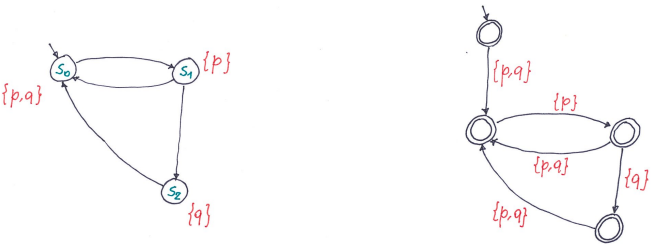
\includegraphics[width=0.5\textwidth]{img/model/kripke-Automa.png}
        \caption{Passaggio da modello di Kripke ad automa}
        \label{fig:kripke-automa}
    \end{figure}
\end{esempio}

Inoltre, per ogni formula LTL è possibile definire un automa di Büchi corrispondente
al modello di Kripke associato alla formula.

Vogliamo ora verificare se una formula $\alpha \in LTL$ è vera nel modello $M$
considerando lo stato $q_0$ ($M, q_0$). Per ottenere questo risultato possiamo
utilizzare il seguente algoritmo:
\begin{enumerate}
    \item Costruiamo l'automa $\mathcal{B}_{\lnot \alpha}$, ovvero l'automa per
          la negazione della formula.
    \item Trasformiamo il modello di Kripke $M$ nell'automa di Büchi equivalente.
    \item Calcoliamo il prodotto sincrono dei due automi ($\mathcal{PS}$, prodotto
          tra automi).
    \item A questo punto se $L(\mathcal{PS}) = \emptyset$, allora $M, q_0 \models
              \alpha$. Se invece tale linguaggio non è vuoto, vuol dire che
          abbiamo trovato un cammino per cui è vera la negazione della formula
          $\alpha$ e quindi $\alpha$ non è vera per quel modello.
\end{enumerate}
\begin{nota}
    Ricorda che Il prodotto sincrono tra automi corrisponde ad un automa che riconosce
    il linguaggio intersezione dei linguaggi accettati dagli automi.
\end{nota}
\section{$\mu$ calcolo}
Il $\mu$ calcolo è un linguaggio logico che permette di definire delle formule
ricorsive.
\begin{esempio}
    Supponiamo di avere un solo operatore temporale $X$. Come possiamo esprimere
    le proprietà $EF \alpha$?
    \begin{equation}
        \begin{array}{ll}
            EF\alpha & \equiv \alpha\lor EX\alpha\lor EXEX\alpha\lor \dots \equiv               \\
                     & \equiv \alpha\lor EX(\alpha\lor EX\alpha\lor EXEX\alpha\lor \dots)\equiv \\
                     & \equiv \alpha \lor EX(EF\alpha)
        \end{array}
    \end{equation}
\end{esempio}
La semantica di questo linguaggio è definita su modelli di Kripke attraverso
gli operatori di punto fisso.

Questo linguaggio ha massima potenza espressiva, ma ha lo svantaggio di avere
un elevata complessità. Questo ci permette di affermare che:
\begin{equation}
    CTL^{\ast} \subset \mu-\text{calcolo}
\end{equation}
In generale questo linguaggio ha un'applicabilità minore vista la sua espressività
e complessità.
\section{Complessità}
Sia $M$ un modello di Kripke e $f$ una formula, e siano $|M|$ il numero di stati
del modello e $|f|$ il numero di simboli nella formula. Allora possiamo definire
la complessità delle logiche definite come:
\begin{itemize}
    \item CTL: $\mathcal{O}(|M| \times |f|)$
    \item LTL: $\mathcal{O}(|M| \times 2^{|f|})$
\end{itemize}
Anche se dalle formule sembrano complessità completamente diverse, il valore di
maggiore peso è composto dalla dimensione del modello, la quale risulta
esponenziale rispetto al numero di stati. Inoltre, le formule LTL sono solitamente
composte da meno simboli rispetto alle formule CTL.
\begin{nota}
    Ricorda che nei sistemi concorrenti gli stati esplodono sempre in un esponenziale.
\end{nota}
Esistono anche altri algoritmi per la dimostrazione di formule:
\begin{itemize}
    \item OBDD: sfruttano i diagrammi di decisione binari ordinati che rappresentano
          le formule in modo simbolico e risparmiano l'esplosione esponenziale
          degli stati.
    \item ordine parziale: si rappresentano i sistemi concorrenti secondo un
          ordine parziale.
    \item SAT: si riduce il problema di dimostrazione a SAT e quindi si sfruttano
          gli algoritmi esistenti per la dimostrazione.
\end{itemize}
\section{Fairness}
Un altro problema dei sistemi concorrenti è che la rappresentazione utilizzata sfrutta
la \textbf{semantica interleaving} che trasforma le relazioni di dipendenza in scelte.
\begin{definizione}[\textbf{Esecuzione unfair}]
    Un'esecuzione è \textbf{unfair} (ingiusta) se un evento rimane abilitato da
    un istante in poi, ma non scatta mai.
\end{definizione}
La possibilità di avere esecuzioni unfair porta a un nuovo problema, ovvero si
vuole limitare la valutazione di una formula all'esecuzione fair.

Possiamo distinguere un esecuzione fair in:
\begin{itemize}
    \item \textbf{Strong fair}: un'esecuzione si dice fortemente fair se:
          \begin{equation}
              GF(t \ \text{abilitata}) \to GF(t \ \text{scatta}) \equiv
              GF(c[t>) \to GF(c[t>c')
          \end{equation}
          ovvero, se un evento $t$ è abilitato infinite volte, allora $t$ scatta
          infinite volte.
    \item \textbf{Weak fair}: un'esecuzione si dice debolmente fair se un evento
          $t$ non è sempre abilitato e le volte che è abilitato non scatta.
\end{itemize}